\chapter{Integrals and Derivatives}
    \section{Fundamental Methods For Evaluating Integrals}
        To evaluate integrals numerically, we will use numerical approximations: the right Riemann sum, the left Riemann sum, or the trapezoidal rule.
        \begin{center}
            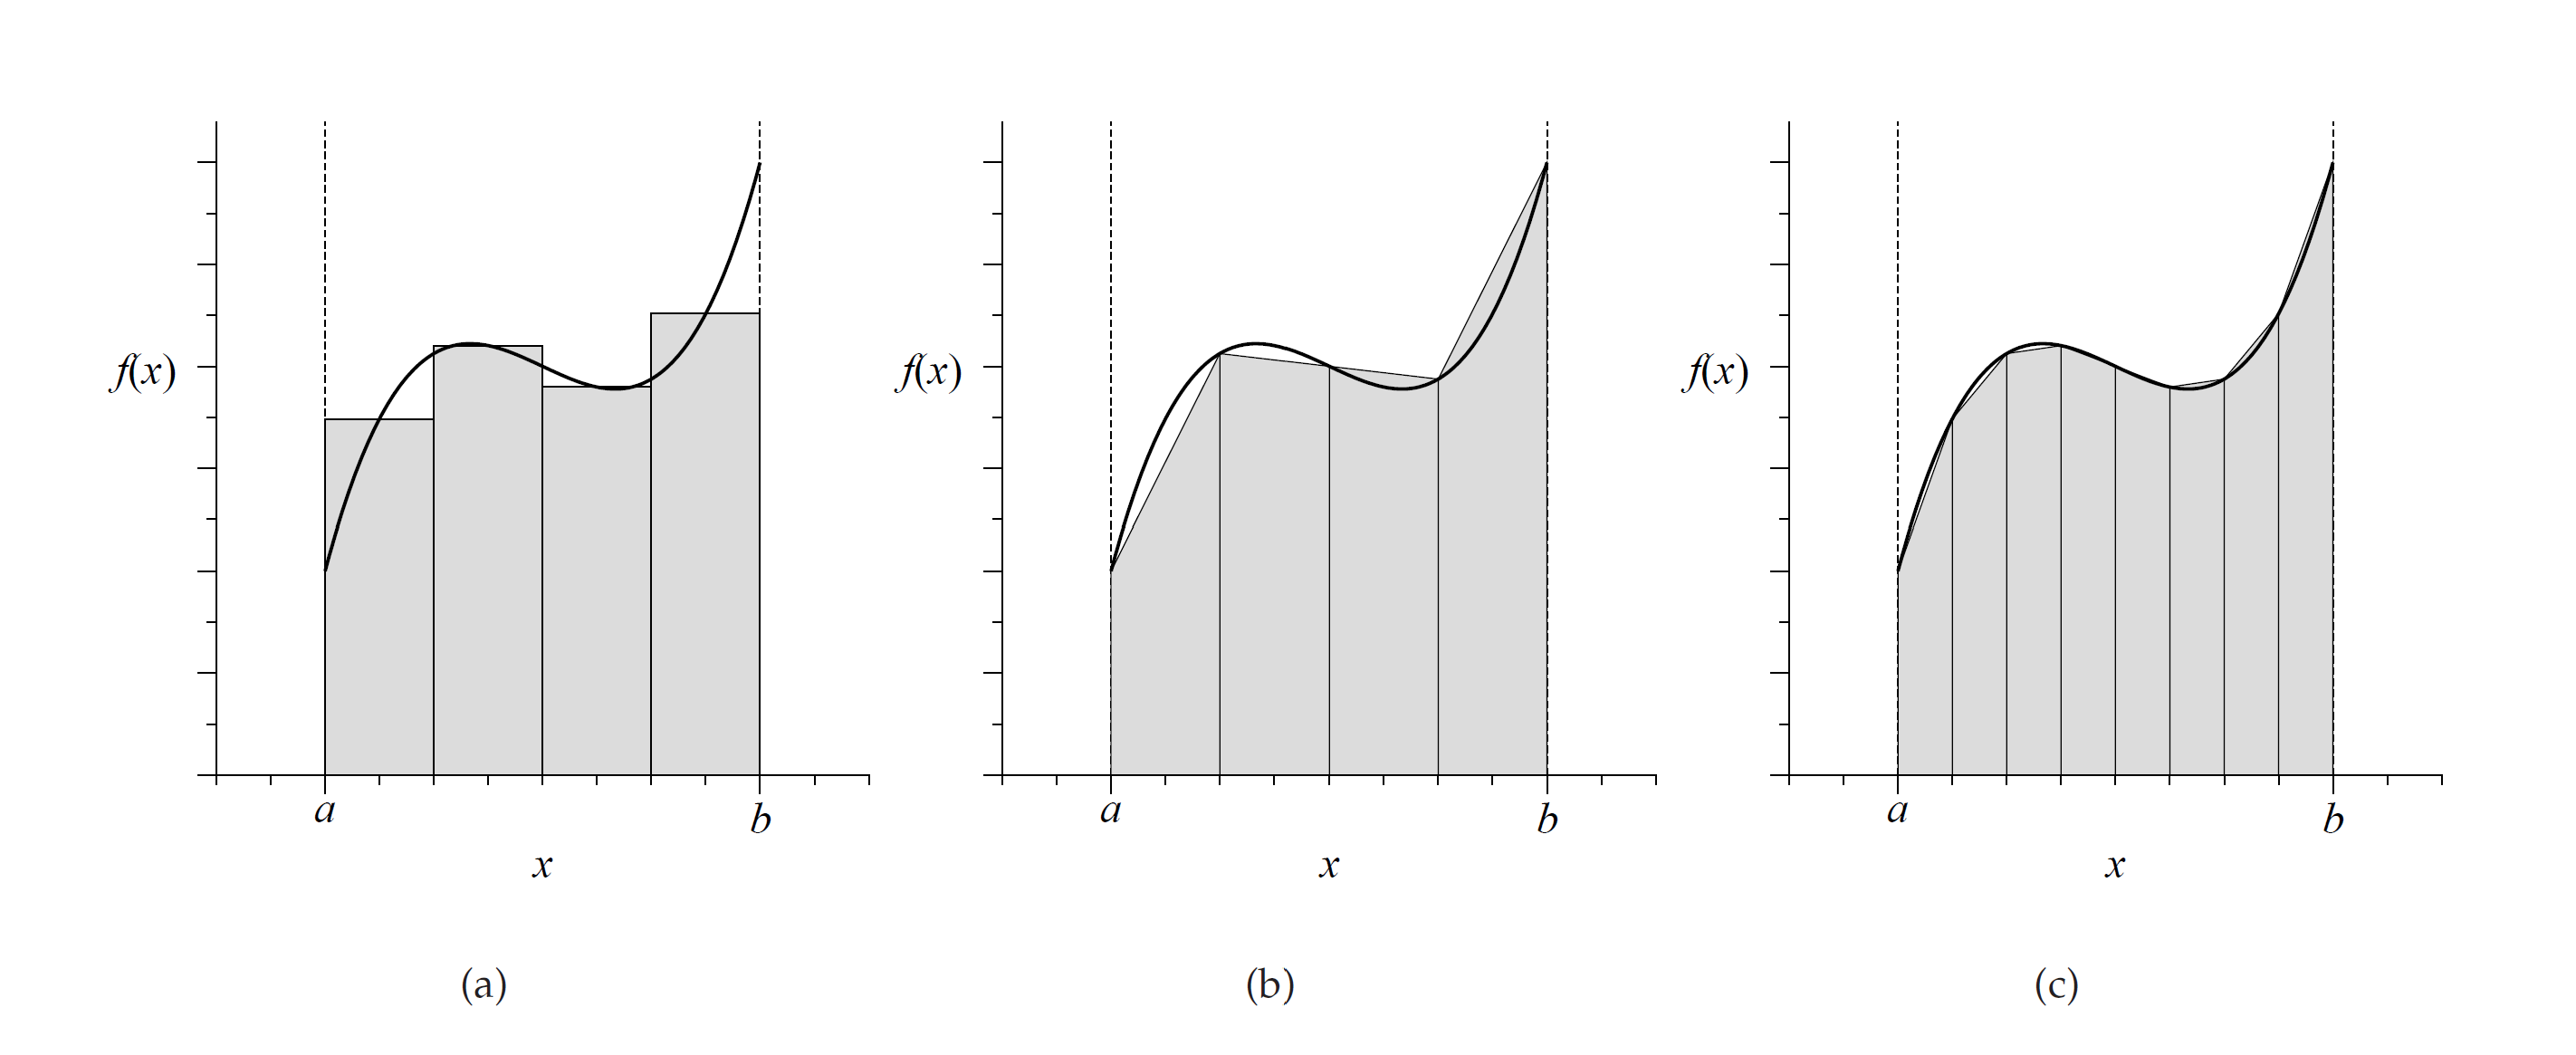
\includegraphics[width=300pt]{integral_approx.png}
        \end{center}
        \subsection{The Trapezoidal Rule}
            Suppose we have a function $f(x)$, let
            \begin{equation*}
                I(a, b) = \int_a^b f(x) dx
            \end{equation*}
            The trapezoidal rule is better than Riemann sums since it is closer to the correct area. Let's divide the interval from $a$ to $b$ into $N$ equal steps so each slice has a width $h = (b - a) / N$. The left and right sides of the trapezoid are $a + (k - 1) h$ and $a + kh$. So the area for slice $k$ is
            \begin{equation*}
                A_k = \frac{1}{2}h[f(a + (k - 1)h) + f(a + kh)]
            \end{equation*}
            Now, our approximation of $I(a, b)$ becomes
            \begin{align*}
                I(a, b) \simeq \sum_{k=1}^N A_k = \frac{1}{2}h \sum_{k=1}^N [f(a + (k - 1)h) + f(a + kh)] \\
                 = h[\frac{1}{2}f(a) + f(a + h) + f(a + 2h) + \dots + \frac{1}{2}f(b)] \\
                 = h[\frac{1}{2}f(a) + \frac{1}{2}f(b) + \sum_{k=1}^{N-1}f(a + kh)]
            \end{align*}
            This is an \textit{extended trapezoidal rule}.